\documentclass[9pt,twocolumn,twoside]{../../styles/osajnl}
\usepackage{fancyvrb}
\journal{i524} 

\title{Apache Derby}

\author[1,*, +]{Ribka Rufael}

\affil[1]{School of Informatics and Computing, Bloomington, IN 47408, U.S.A.}


\affil[*]{Corresponding authors: rrufael@umail.iu.edu}

\affil[+]{HID: S17-IO-3016}

\dates{paper2, \today}

\ociscodes{Apache Derby, relational database management system, JDBC}

% replace this with your url in github/gitlab
\doi{\url{https://github.com/cloudmesh/sp17-i524/blob/master/paper2/S17-IO-3016/report.pdf}}


\begin{abstract}

  Apache Derby, part of Apache DB subproject, is Java based relational
  database management system. Apache Derby database provides storage,
  access and secure management of data for Java based
  applications. Apache Derby is an open source software and it is
  licensed under Apache version 2.0. Apache Derby is written in Java
  and it runs on any certified JVM(Java Virtual Machine). JDBC driver
  in embedded or netwrok server frameworks allows applications to
  access Apache Derby Database.
 \newline
\end{abstract}
\setboolean{displaycopyright}{true}

\begin{document}

\maketitle

\section{Introduction}

Apache Derby is an open source relational database management
system(RDBMS). Applications interact with Apache Derby database
through JDBC(Java Database Connectivity) driver. Apache Derby is built
in Java programming language which makes it platform
independent. Apache Derby can be embedded into Java based application
or it can be setup to run in a client/server environment. Apache Derby
complies with JDBC and ANSI SQL standards. Apache Derby database
allows applications to create, update, read, delete and manage data
\cite{www-derbyoverview,www-apachederbycharter}.

Apache Derby is part of the Apache DB subproject of Apache Software
Foundation. It was in August 2004 that IBM submitted the Derby code to
Apache Software Foundation. Then Apache Derby became part of the
Apache DB project in July 2005 \cite{www-apachederbycharter}.

\section{Architecture}

There are two views that describe Apache Derby's architecture. These
views are Module View and Layer/Box view \cite{www-derbyarch}.

\subsection {Module View} 


Modules and Monitor are components in Apache Derby database system. A
collection of distinct functionality is a module. Examples of modules
in Apache Derby are lock management, error logging and JDBC
driver. Lock management is responsible for controlling concurrent
transactions on data objects. Once Apache Derby database is up and
running any informational messages or error messages are logged. This
message logging is handled by error logging module.  Applications use
JDBC driver to interact with Apache Derby database. A number of
classes are used for the implementation of each module
\cite{www-derbyarch}.

The monitor is responsible for managing Apache Derby
database. Whenever request to modules come, the monitor is responsible
for selecting appropriate module implementation depending on what the
module request was and from which environment the request came from
\cite{www-derbyarch}.

\subsection{Layer/Box View} 

JDBC, SQL, Store and Services are the four layers in Apache Derby. The
Java Database Connectivity abbreviated JDBC is an API(Application
Programming Interface) which allows applications to connect to Apache
Derby database. JDBC interfaces that Apache Derby implements allow
applications to connect to Apache Derby. Some of the interfaces are
Driver, DataSource, ConnectionPoolDataSource, XADataSource and
PreparedStatement. Apache Derby JDBC has implementation of java.sql
and javax.sql classes \cite{www-derbyarch}.

The other layer which sits below JDBC is SQL layer. Compilation and
execution are the two logical parts of SQL layer. SQL statement that
is invoked by an application to Apache Derby Database passes through
five step compilation process. First statement is parsed with a parser
created by JavaCC(Java Compiler Compiler) and tree of query nodes is
created, second step is binding to resolve objects , third step is
optimizing to identify the access path, in fourth step Java class is
created for the statement this is then cached to be used by other
connections and finally class is loaded and instance of generated
statement is created. During execution, execute methods on the class
instance created during compilation are called and Derby result set is
returned. JDBC layer is responsible in converting the Derby result set
into JDBC result set for the applications \cite{www-derbyarch}.

Access and raw are the two parts of the store layer. Raw data storage
for data in files and pages, transaction logging and management is
handled by the raw store. The access store interfaces with SQL layer
and takes care of scanning of tables and indexes, indexing, sorting,
locking and etc \cite{www-derbyarch}.

Lock management, error logging and cache management are part of the
service layer. Clock based algorithm is used by cache management. It
is mainly used for caching buffer, caching compiled java classes for
SQL statement implementation plans and caching table descriptors
\cite{www-derbyarch}.

\subsection{Shell Access}

Shell access to Apache Derby database is achieved by ij. ij is one of
java utility tools that allows performing sql scripts on Derby
database in embedded or network server frameworks. ij tool can be used
for creating database, connecting to database, run and execute sql
scripts.  Commands in ij are case sensitive and semicolon is used to
mark end of command.  Other utility tools that come with Apache Derby
are sysinfo , dblook and SignatureChecker. sysinfo is used to get
version and other information about Apache Derby and the Java
environment. dblook utility is used to generate Data Definition
Language(DDL) for Derby database. Checks, functions, indexes, jar
files, primary keys, foreign keys and schemas are the objects
generated by dblook.  SignatureChecker is used to check whether
functions and procedures used in Derby database comply with the rules
and standards \cite{www-derbyutil}.

\subsection{API}

Applications can interact with Apache Derby database through two JDBC
drivers org.apache.derby.jdbc.EmbeddedDriver and
org.apache.derby.jdbc.ClientDriver for embedded and network server
frameworks respectively \cite{www-derbyutil}.



\section {Installation}

Java 2 Standard Edition (J2SE) 6 or higher is needed for installing
Apache Derby and for running Derby the Java Runtime Environment (JRE)
is needed. Apache Derby can be downloaded from the Apache DB download
page \cite {www-derbydownload}. Apache Derby can be installed on
Windows, MAC, UNIX and Linux operating systems. After downloading the
zipped installation file, the file should be extracted into directory
and then DERBY\textunderscore INSTALL variable should be set in the
same directory as where Derby was installed. Apache Derby provides two
frameworks Embedded Derby and Derby Network Server \cite
{www-derbytutorial}.

\subsection{Embedded Derby}
In the embedded Derby framework, Apache Derby engine and the
application which accesses it run on the same JVM(Java Virtual
Machine). Embedded Derby JDBC driver is used by the application to
interact with Apache Derby database. To setup Embedded Derby mode,
derby.jar and derbytools.jar must be included in the CLASSPATH after
installation. The Derby engine and Embedded Derby JDBC driver are
included in derby.jar. derbytools.jar includes ij tool( utility tool
which can be used as scripting tool to interact with Derby
database). In Embedded Derby framework, multiple users that are
running in the same JVM can access the same database. Figure 1 shows
the Embedded Derby framework \cite {www-derbytutorial}.

\begin{figure}[htbp]
\fbox{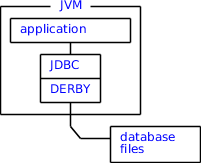
\includegraphics[scale=0.55]{images/embeddedDerby.jpg}}
\caption{Embedded Derby Framework  \cite {www-derbytutorial}.}
\end{figure}


\subsection{Derby Network Server}
Derby Network Server framework allows multiple application running
in the same JVM or different JVMs to access Derby database over the
netwrok in a typical client/server architecture. In this framework
application accesses Derby database through Derby Network Client JDBC
driver. To setup Derby netwrok server derbynet.jar and derbytools.jar
must be included in CLASSPATH on the server side. The program for
Network Server and reference to the Derby engine are included
derbynet.jar file. On the client side, derbyclient.jar and
derbytools.jar must be included in CLASSPATH. Derby Network Client
JDBC driver is included in derbyclient.jar file. Derby Network Server
listens and accepts requests on port 1527 by default but this can be
changed to a different port if needed. Figure 2 shows the Derby
Network Server framework \cite {www-derbytutorial}.

\begin{figure}[htbp]
\fbox{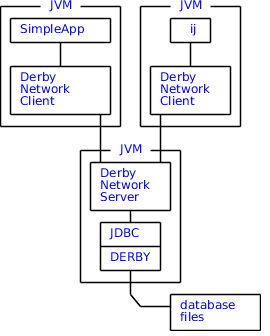
\includegraphics[scale=0.45]{images/networkserverDerby.jpg}}
\caption{Derby Network Server Framework  \cite {www-derbytutorial}.}
\end{figure}

Another variation for setting up Derby Network Server is embedded
server. In embedded server, application will have both Embedded Derby
JDBC driver and Network Server. The application uses Embedded Derby
JDBC driver which runs on the same JVM and extends access to other
applications running on different JVMs through the Network Server
\cite {www-derbytutorial}.

\section{Security}

Apache Derby provides a number of security options. Some of these
features are authentication, authorization and disk encryption.
Before users are granted access to the Derby database, Derby can be
setup to perform user authentication. There may be a need for certain
user groups to have read only access to Derby database and some other
user groups to have both read and write access to Derby database which
can be achieved by Derby's user authorization feature. Data which is
saved on disk can be encrypted with Derby's disk encryption feature
\cite {www-derbysec}.

\section{Use Cases}

Apache Hive, data warehouse querying and analysis software, uses
Apache Derby database by default for metadata store.  Apache Derby can
be configured in the embedded or netwrok server mode for Hive meta
data storage \cite {www-hive, www-hivemetastore}.

My Money, management and analysis software for personal and business
finances which is built by MTH Software, Inc, uses Apache Derby as a
relational database management system \cite {www-mymoney,
  www-mymoneywiki}.

\section{Licensing}

Apache Derby is an open source technology hence it is available for
free. Apache Derby is licensed under Apache License, Version 2.0
\cite {www-derbyoverview}.

\section {Educational Material}

Apache Derby tutorial page is one of the resources which can be used
by users who are new to Apache Derby. This tutorial contains step by
step information about Apache Derby installation, embedded framework
configuration and network server framework configuration \cite
{www-derbytutorial}. Derby Engine Architecture Overview page provides
information about Apache Derby architecture \cite
{www-derbyarch}. Apache Derby documentation page has list of
documentations that can be used as reference for new users, developers
and administrators \cite {www-derbdoc}.

\section {Conclusion}

Apache Derby database offers storage,access and secure management of
data for Java based applications. Apache Derby provides complete
relational database management package that complies with JDBC and
ANSI SQL standards. Apache Derby's small size makes it suitable for
embedding it into applications which run on smaller devices with less
physical memory. As the use case of Hive using Apache Derby for
metadata storage indicates, Apache Derby can be incorporated into
software stack for big data projects for metadata storage.

\section*{Acknowledgements}

The author would like to thank Professor Gregor von Laszewski and
associate instructors for their help and guidance.


% Bibliography

\bibliography{references}
\newpage
\appendix
\end{document}
